\subsection*{\textit{\textbf{RQ4: What are the most influential attributes for
modeling delivery delay?}}}

\subsubsection*{\textit{\textbf{RQ4: Results for delivery delay in terms of
releases}}}

\noindent\textit{\textbf{The fixing time per resolver and integration workload
attributes are the most influential attributes in our models.}}
\hyperref[ch4:fig:variableImportance]{Figure}~\ref{ch4:fig:variableImportance} shows the
variable importance values of the LOOCV of our models. The most influential
attribute is the \textit{fixing time per resolver}. The \textit{fixing time per
resolver} attribute measures the total time that is spent by each resolver on
fixing issues in a release cycle. The second most influential attributes are
integration workload attributes (\ie backlog of issues and backlog of issues per
resolver). These integration workload attributes measure the competition of
issues that were addressed but not yet integrated into an official release.

\begin{figure}
	\center
	\subfloat[Eclipse]{
		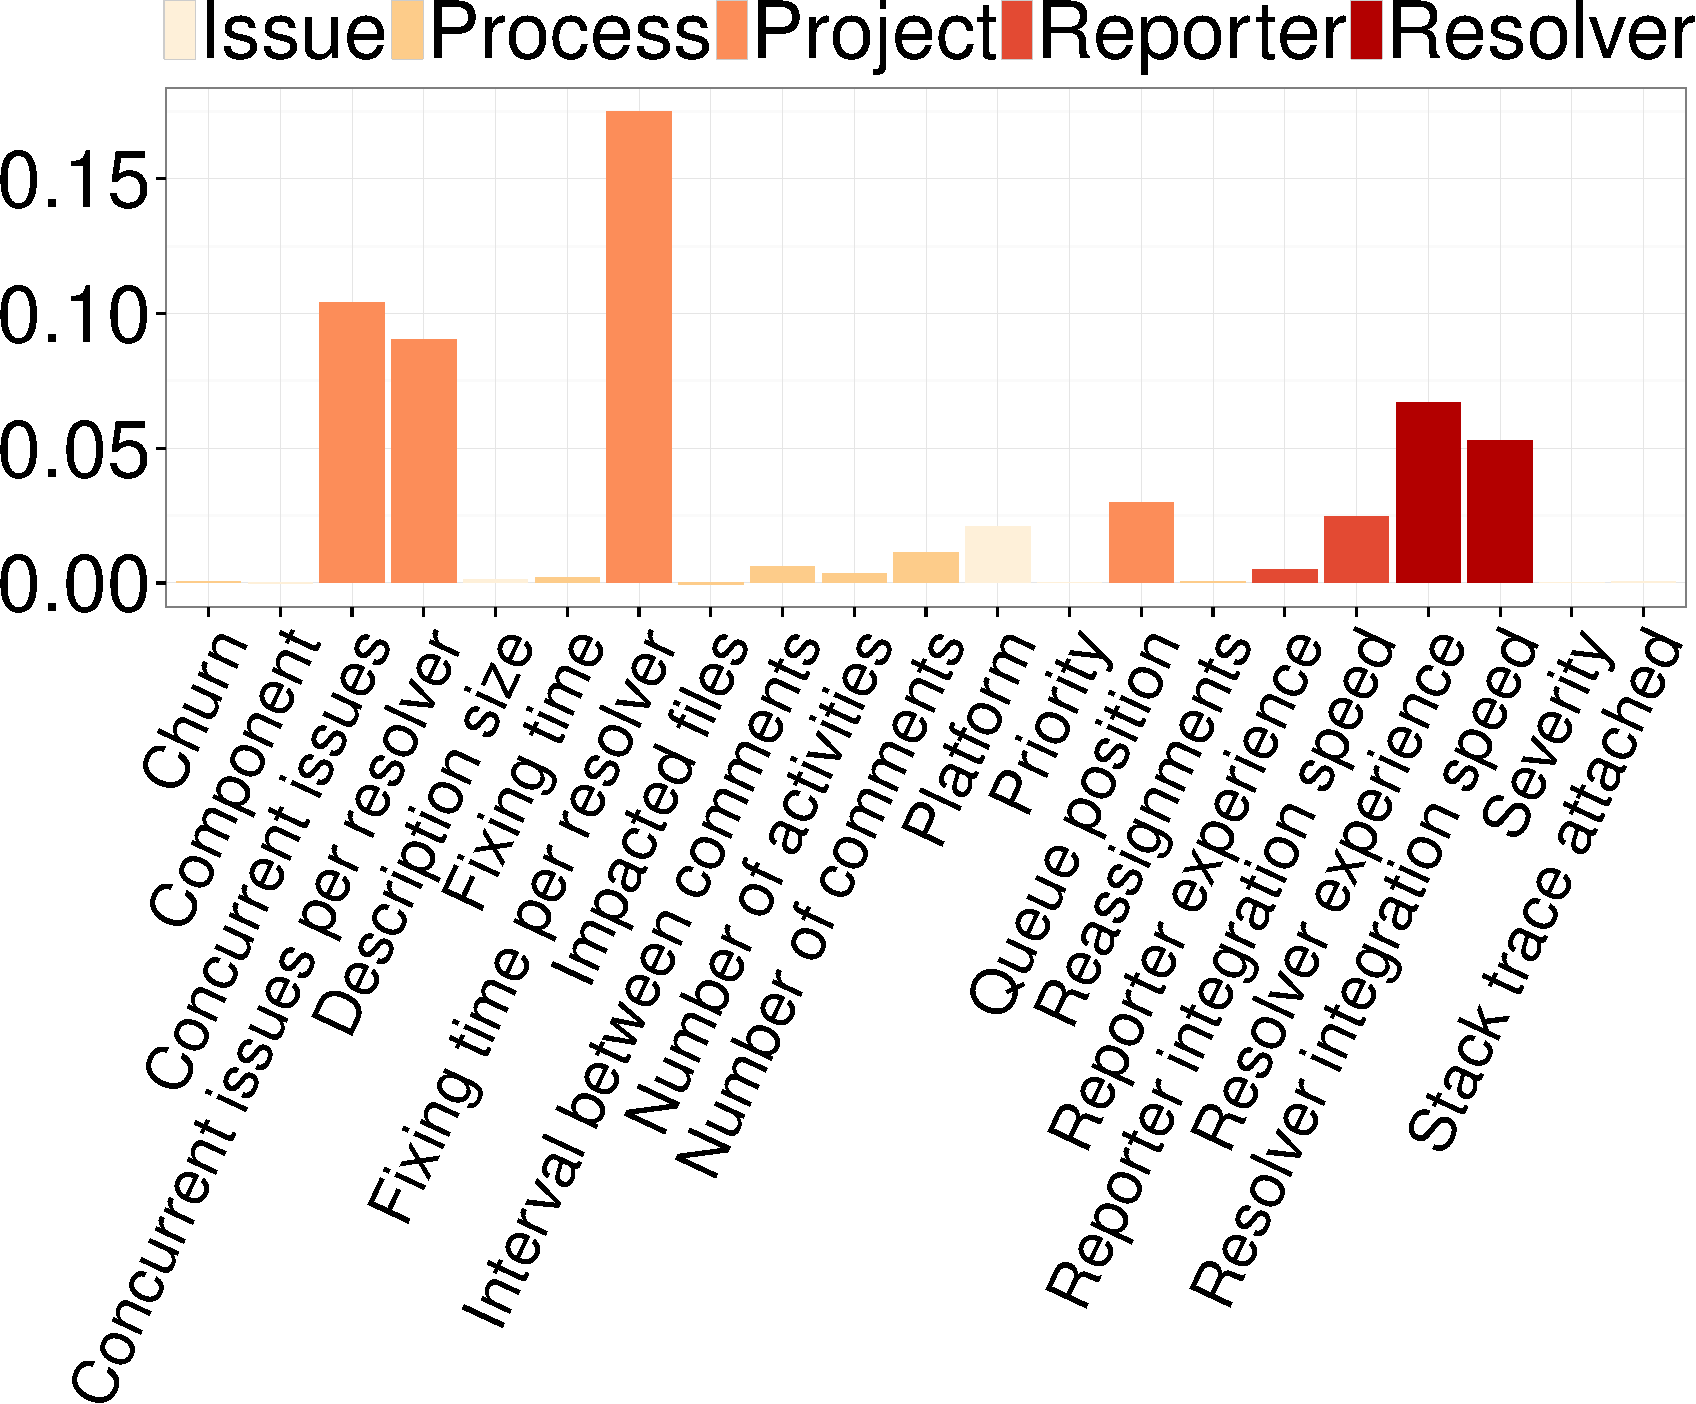
\includegraphics[width=0.55\textwidth,keepaspectratio] 
		{chapters/chapter4/figures/eclipse_loocv_varimp.pdf}
	\label{ch4:fig:impEclipse}
	}

	\subfloat[Firefox]{
		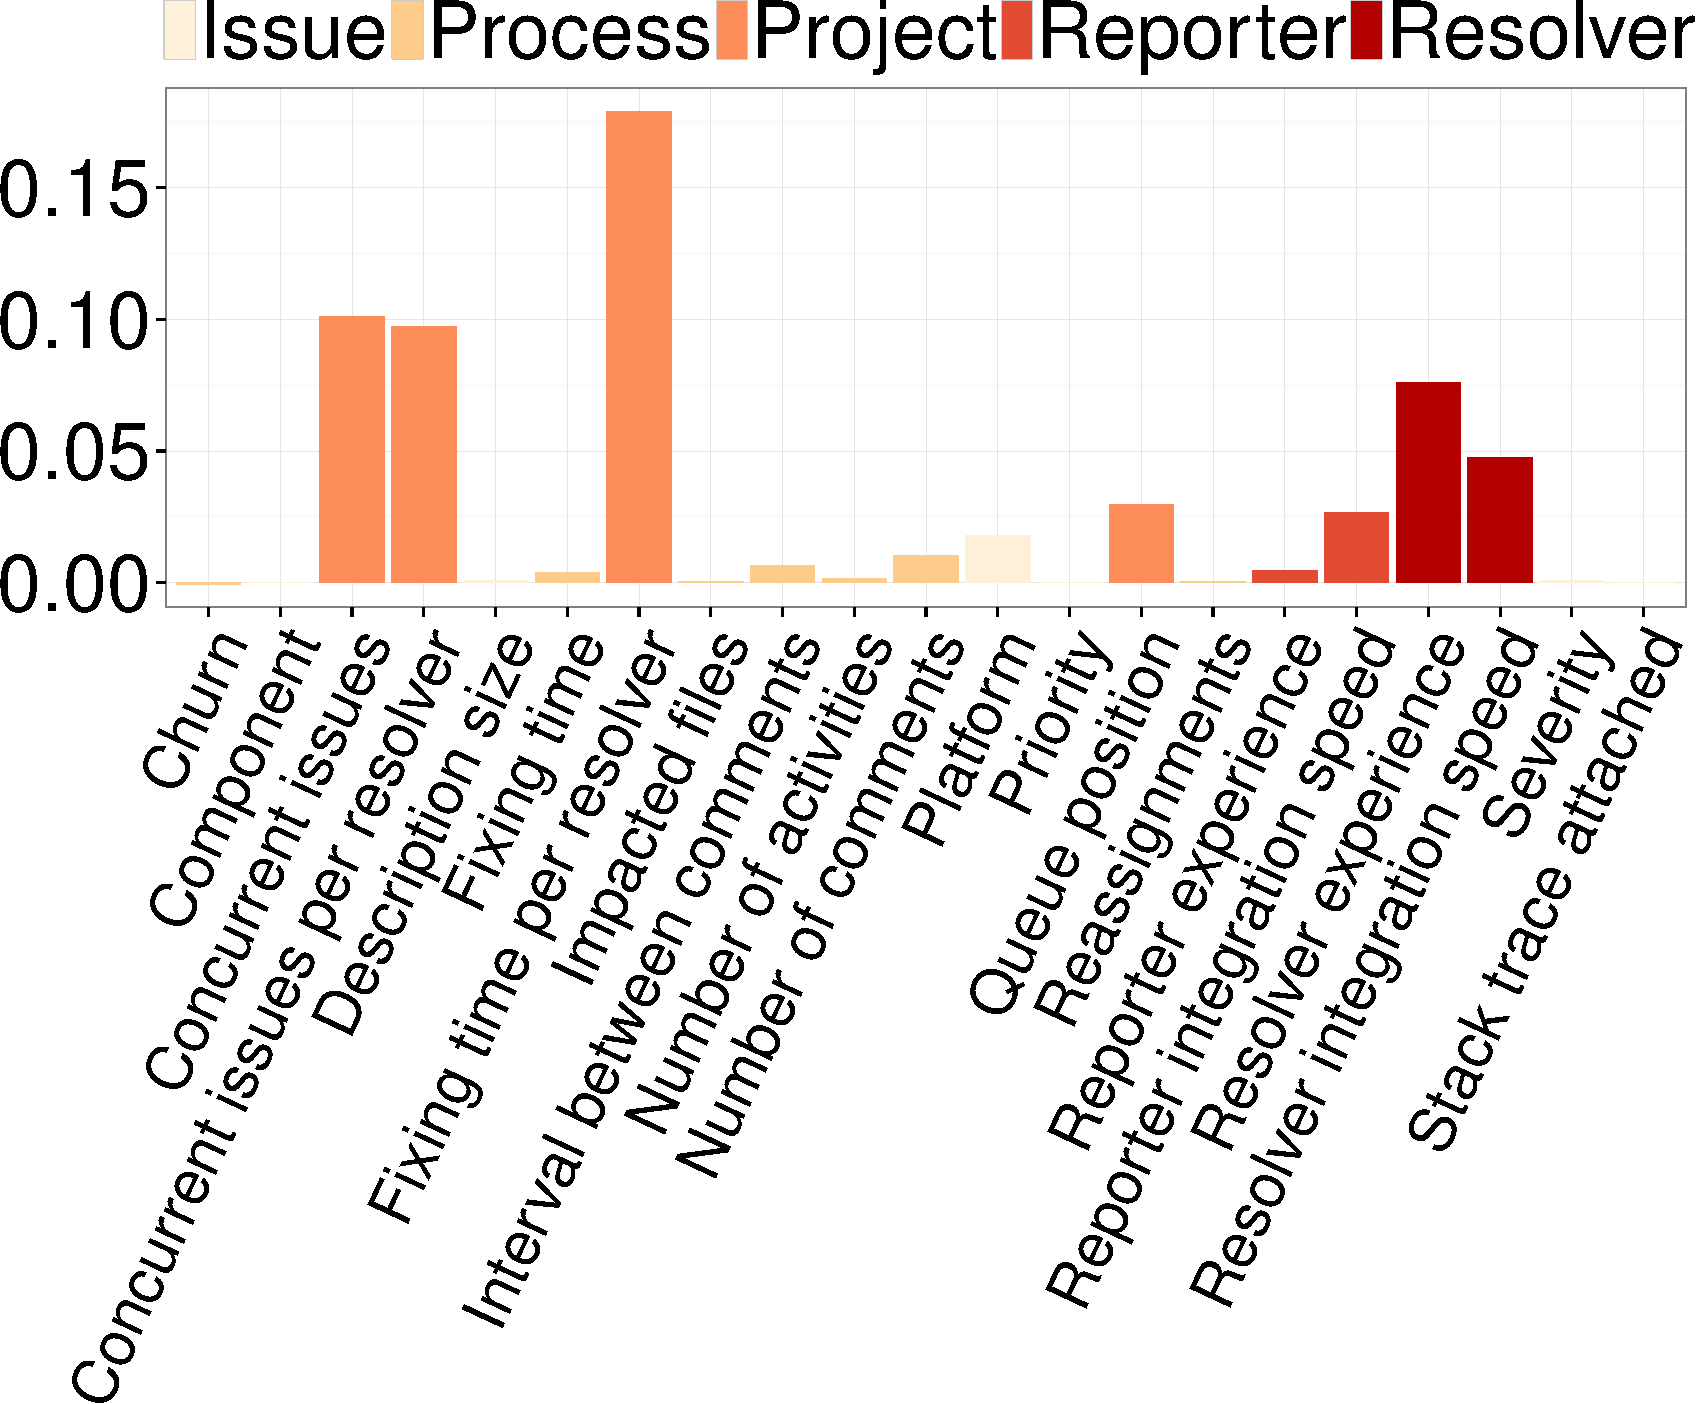
\includegraphics[width=0.55\textwidth,keepaspectratio]  
		{chapters/chapter4/figures/firefox_loocv_varimp.pdf}
		\label{ch4:fig:impFirefox}
	}

	\subfloat[ArgoUML]{
		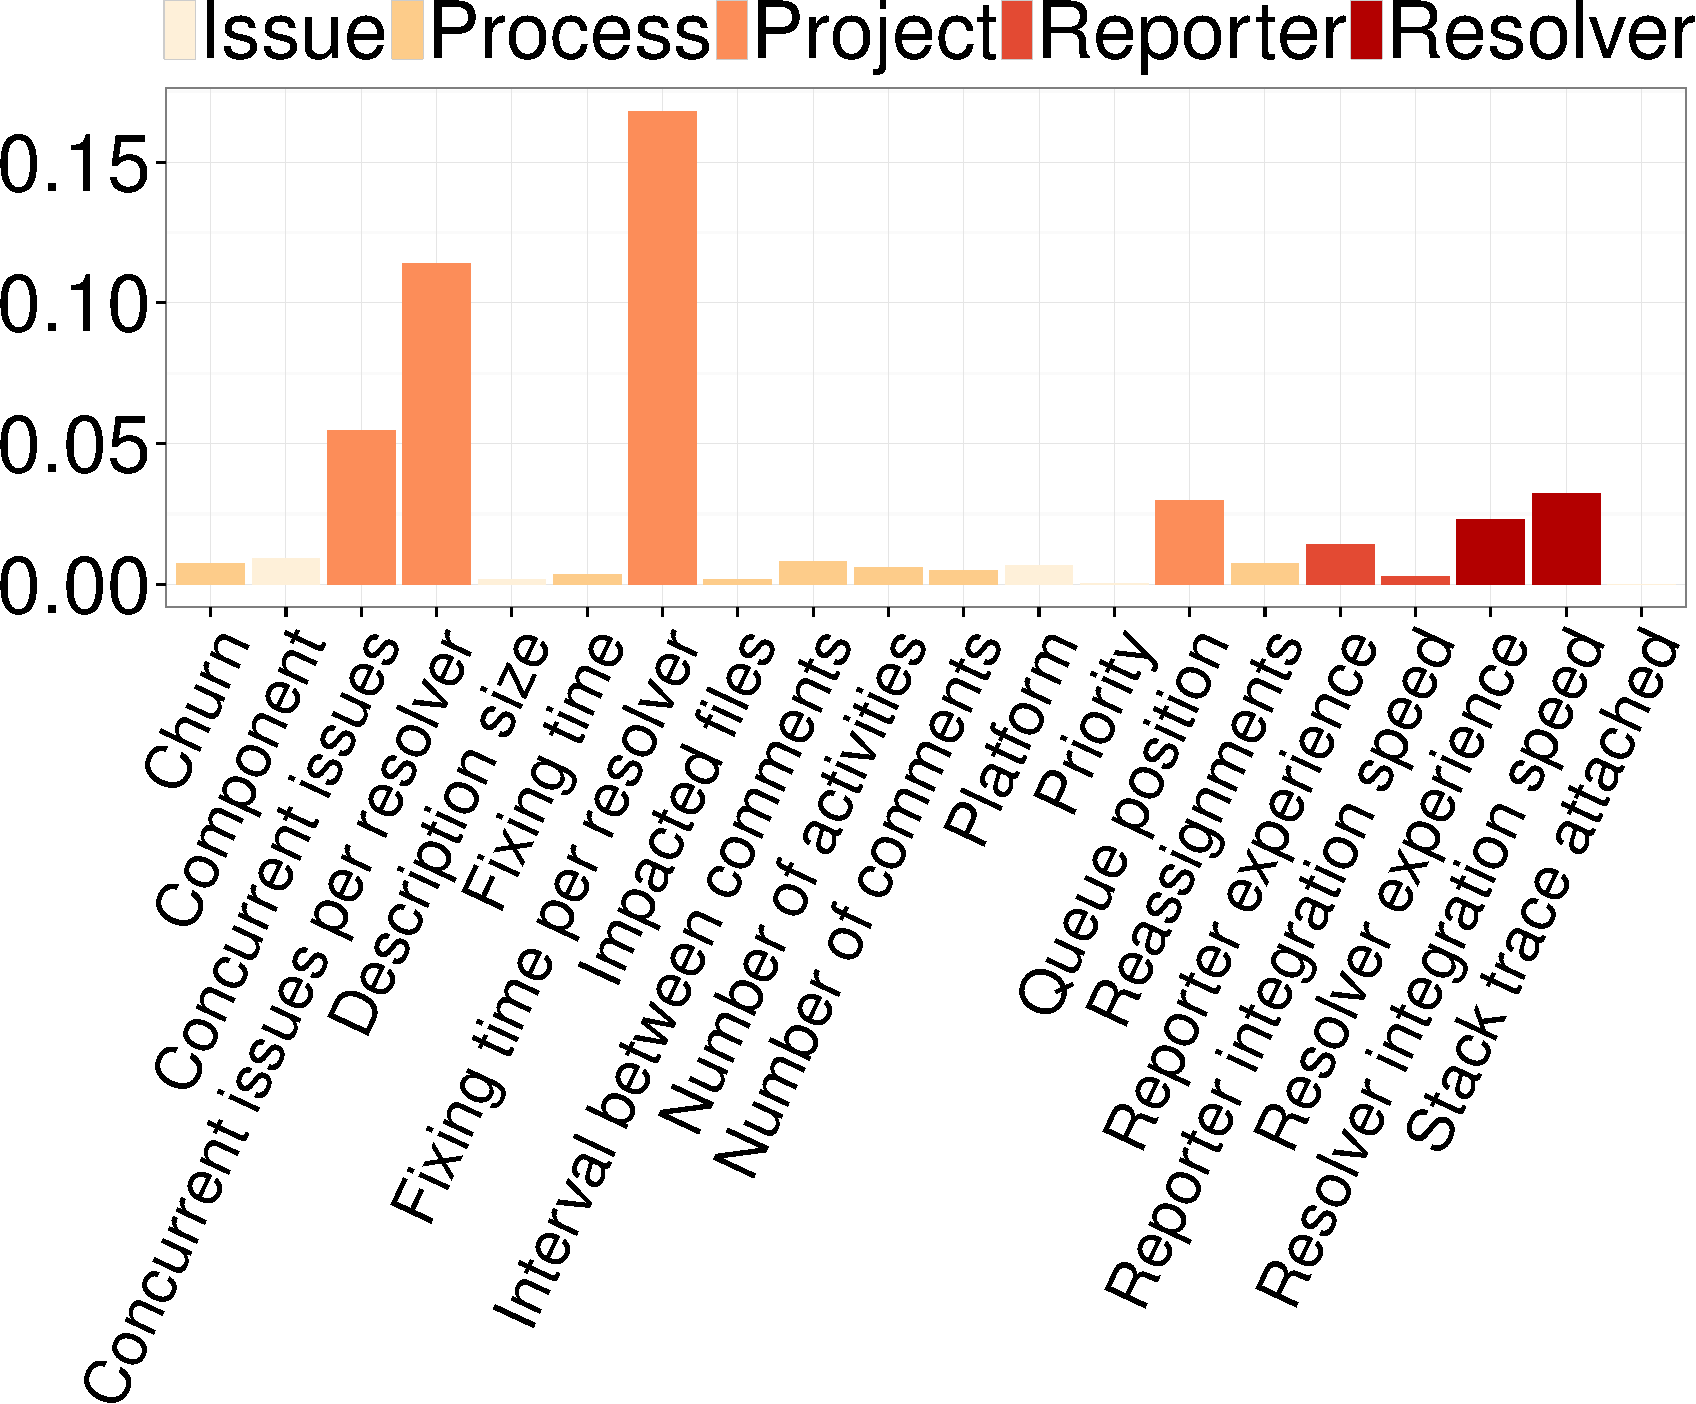
\includegraphics[width=0.55\textwidth,keepaspectratio] 
		{chapters/chapter4/figures/argouml_loocv_varimp.pdf}
	\label{ch4:fig:impArgo}}
	\caption{\textbf{Variable importance scores.} We show the 
		importance scores that are computed for the LOOCV of our models.}
	\label{ch4:fig:variableImportance}
\end{figure}

Our results suggest that the time that is invested by the resolvers on fixing
issues have a strong association with delivery delay. This could be due to
resolvers fixing issues more carefully---which would lead to a smoother
integration of such issues---or issues that were less complex in overall (\eg a
shorter time was invested), which might simplify the integration process. A deeper
analysis of this attribute would be necessary to better understand the exact
reasons behind this relationship (\eg consulting the development team through
surveys and interviews). 

We also observe that integration workload attributes (\ie \textit{backlog of
issues} and \textit{backlog of issues per resolver}) are the second most
influential attributes in the three studied projects. This finding suggests that
the integration backlog introduces overhead that may lead to longer integration
time.

\begin{figure}[!t]
	\centering
	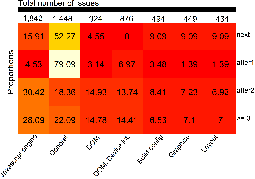
\includegraphics[width=0.60\textwidth,keepaspectratio]
	{chapters/chapter4/figures/firefox/RQ3_component_hm.pdf}
	\caption{\textbf{The spread of issues among the Firefox components.} The
		darker the colors, the smaller the proportion of issues that
	impact that component.}
	\label{ch4:fig:componentHeatmap}
\end{figure}

Furthermore, we study the distribution of addressed issues across components in the
Firefox project.
\hyperref[ch4:fig:componentHeatmap]{Figure}~\ref{ch4:fig:componentHeatmap} shows the top
seven components of the Firefox project, each having more than 400 addressed issues.
We analyze the proportion of addressed issues where integration was prevented in the
top seven components.
\hyperref[ch4:fig:componentHeatmap]{Figure}~\ref{ch4:fig:componentHeatmap} shows that,
for buckets \textit{next} and \textit{after-1}, the majority of issues are
related to the \textit{General component}, whereas for \textit{after-2} and
\textit{after-3-or-more} the majority are related to the \textit{Javascript
engine} component. Addressed issues related to the \textit{General} component
may be easy to integrate, whereas issues related to the \textit{Javascript
Engine} may require more careful analysis before integration.  \\


\noindent\textit{\textbf{Severity and priority have little influence on
delivery delay in terms of releases.}} Users and contributors of software
projects can denote the importance of an issue using the \textit{priority} and
\textit{severity} fields. Previous studies have shown that priority and
severity have little influence on bug fixing time
\cite{tian2015unreliability,Herraiz2008,Mockus:2002}. For example, while an
issue might be severe or of high priority, it might be complex and would take a
long time to fix.  

However, in the integration context, we expect that priority and severity would
be more influential, since the issues have already been addressed. Even though
priority and severity are often left at their default values (see
\hyperref[ch4:sec:subjects]{Section}~\ref{ch4:sec:subjects}), one would expect that the
integrators would fast-track the integration of issues for which they
care about increasing the levels of severity or priority. For instance,
according to the Eclipse project guidelines for filing issue reports, a priority
level of P1 is used for serious issues and specifies that the existence of a P1
issue should prevent a release from
shipping.\smartfoot{\url{http://wiki.eclipse.org/Development_Resources/HOWTO/Bugzilla_Use}}
Hence, it is surprising that priority and severity play such a small role in
determining the release in which an addressed issue will appear. Indeed,
\hyperref[ch4:fig:variableImportance]{Figure}~\ref{ch4:fig:variableImportance} shows
that the priority and severity metrics obtain low importance scores.

\begin{figure}
	\centering
	%\captionsetup{justification=centering}
	\subfloat[ArgoUML Priority]{
		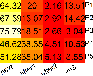
\includegraphics[width=0.30\textwidth,keepaspectratio] 
		{chapters/chapter4/figures/argouml/RQ3_priority_hm.pdf}
	\label{ch4:fig:heatMap_argo}}
	\subfloat[Eclipse Priority]{
		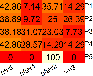
\includegraphics[width=0.30\textwidth,keepaspectratio] 
		{chapters/chapter4/figures/eclipse/RQ3_priority_hm.pdf}
	\label{ch4:fig:heatMap_eclipsep}}
	\subfloat[Firefox Priority]{
		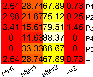
\includegraphics[width=0.30\textwidth,keepaspectratio]  
		{chapters/chapter4/figures/firefox/RQ3_priority_hm.pdf}
		\label{ch4:fig:heatMap_firefoxp}
	}

	\subfloat[Eclipse Severity]{
		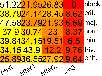
\includegraphics[width=0.35\textwidth,keepaspectratio] 
		{chapters/chapter4/figures/eclipse/RQ3_severity_hm.pdf}
	\label{ch4:fig:heatMap_eclipses}}
	\subfloat[Firefox Severity]{
		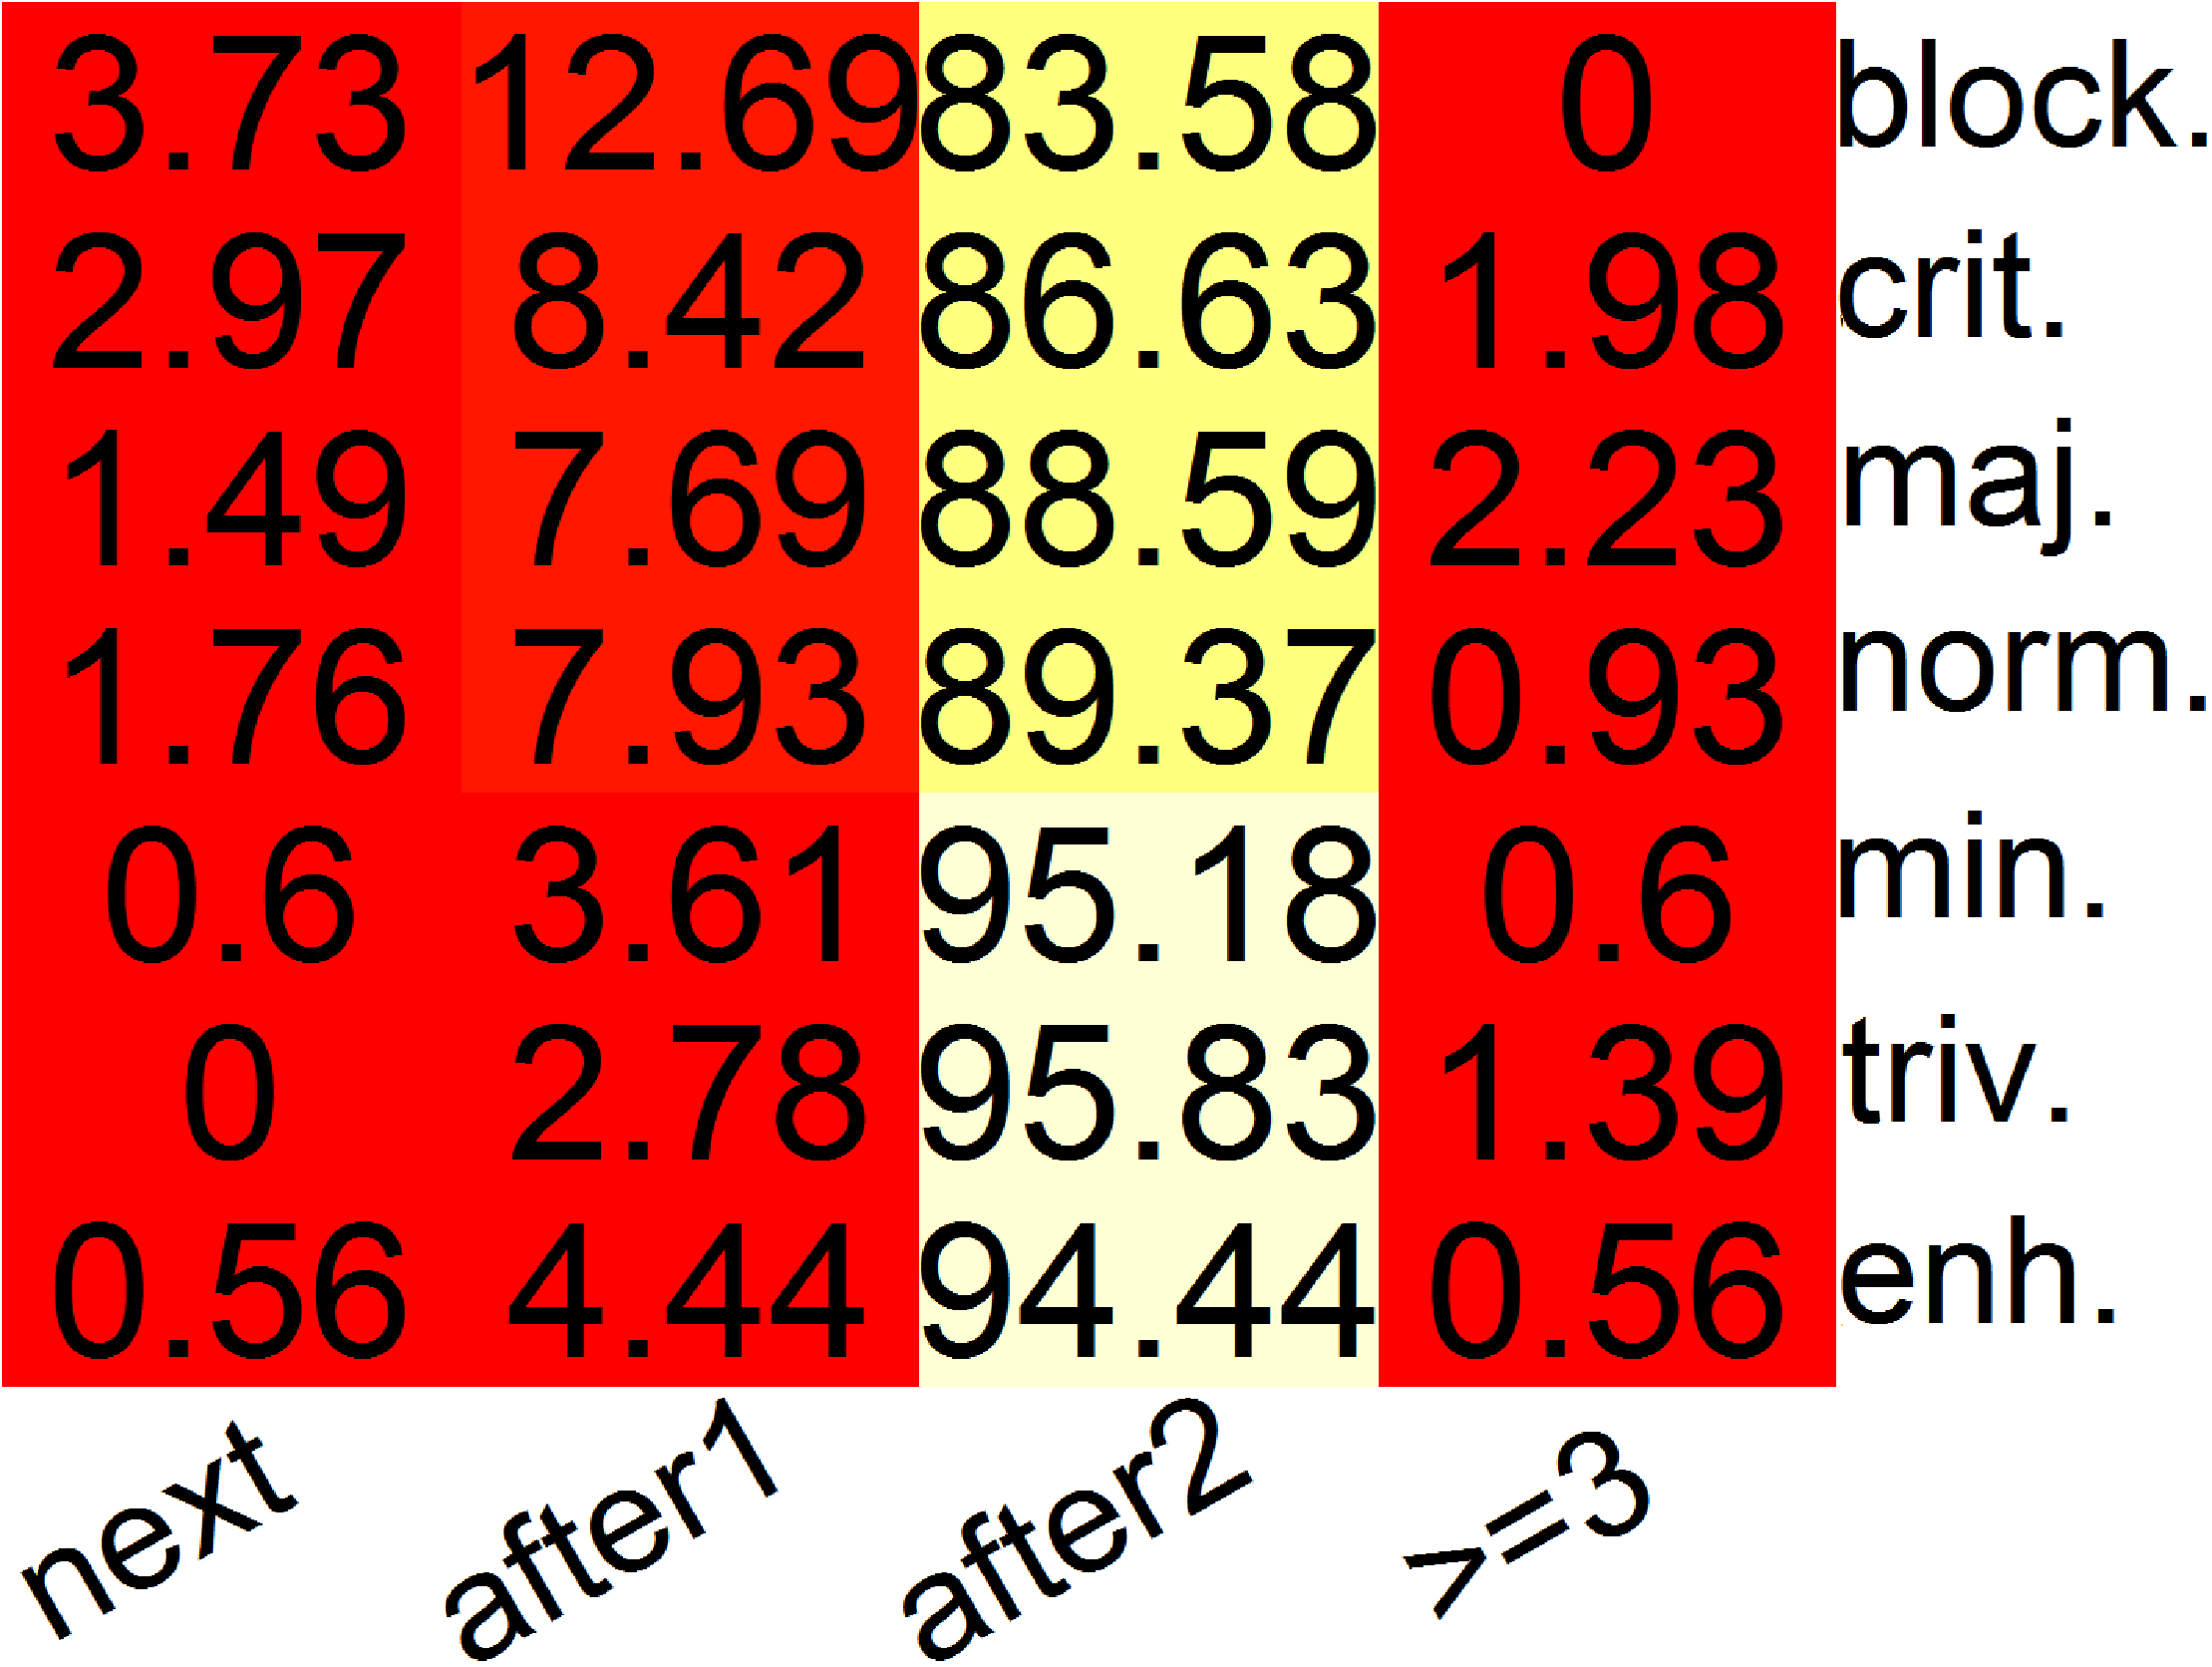
\includegraphics[width=0.35\textwidth,keepaspectratio]  
		{chapters/chapter4/figures/firefox/RQ3_severity_hm.pdf}
		\label{ch4:fig:heatMap_firefoxs}
	}
	\caption{\textbf{The percentage of priority and severity levels in each
		studied bucket of delivery delay.} We expect to see light
		colour in the upper left corner of these graphs, indicating that
		high priority/severity issues are integrated rapidly.
	Surprisingly, we are not seeing such a pattern in our datasets.}
	\label{ch4:fig:heatMaps}
\end{figure}

\hyperref[ch4:fig:heatMaps]{Figure}~\ref{ch4:fig:heatMaps} shows the percentage of
issues with a given priority (\textit{y-axis}) in a given integration bucket
(\textit{x-axis}). The integration of 36\% to 97\% of priority P1 addressed issues
had their integration prevented in at least one release, whereas the integration
of 32\% to 96\% of priority P2 addressed issues were prevented from integration in
at least one release. 

In the ArgoUML project, while the majority of priority P1 issues (64\%) were
integrated in the \textit{next} release, 36\% of them had their integration
prevented in at least one release. For the Firefox project, 97\% of the P1
issues and 96\% of the \textit{blocker} issues were prevented from integration
in at least one release. Finally, for the Eclipse project, 57\% of P1 issues and
49\% of blocker issues had their integration prevented in at least one release.
Hence, our data shows that, in the context of issue integration, the
\textit{priority} and \textit{severity} values that are recorded in the ITSs
have little influence on delivery delay. Instead, addressed issues might be
prioritized by the level of risk that are associated to
them.\smartfoot{Two issues from our sample were
	promoted to stabler release channels due to low associated risk \url{https://bugzilla.mozilla.org/show_bug.cgi?id=724145} and
\url{https://bugzilla.mozilla.org/show_bug.cgi?id=732962}, while another issue was prevented from integration due to code break
\url{https://bugzilla.mozilla.org/show_bug.cgi?id=723793}.} This might explain
why the time that is invested on fixing issues during a release cycle reduces
delivery delay---a risk of an addressed issue breaking the code would be
smaller when more time is invested at fixing activities. 

\conclusionbox{The total time that is invested in fixing issues of a release
	cycle and integration workload attributes are the most influential
	attributes in our models. We also find that priority and severity have
	little influence in estimating delivery delay.}

\subsubsection*{\textbf{\textit{RQ4: Results for delivery delay in terms of days}}}

\begin{table}[t]
	\scriptsize
	\centering
	\caption{\textbf{Explanatory power of attributes.} We present the
		$\chi^2$ proportion and the degrees of freedom that are spent
		for each attribute. The $\chi^2$ of the two most influential
		attributes of each model are in bold.
	\label{ch4:tbl:explanatory_power}}
	\begin{threeparttable}
		\begin{tabular}{llrrr}
			\cline{3-5} 
			\multicolumn{2}{c}{} & 
			Eclipse &
			Firefox &
			ArgoUML
			\tabularnewline
			\hline
			\multicolumn{2}{l}{Wald $\chi^2$} & 
			$1,180$ &
			$8,560$ &
			$2,803$
			\tabularnewline
			\hline 
			\multicolumn{2}{l}{Budgeted Degrees of Freedom} &
			$87$ & 
			$879$ &
			$102$
			\tabularnewline
			\hline
			\multicolumn{2}{l}{Degrees of Freedom Spent} &
			$24$ & 
			$33$ &
			$28$
			\tabularnewline
			\hline 
			\multirow{2}{*}{Reporter experience} & 
			D.F. & 
			$1$ & 
			$1$ &
			$1$
			\tabularnewline 
			& 
			$\chi^2$ & 
			$4^{\ast\ast\ast}$ &  
			$\approx 0$ &
			$1^{\ast\ast}$
			\tabularnewline
			\hline 
			\multirow{2}{*}{Resolver experience} & 
			D.F. & 
			$1$ & 
			$1$ &
			$1$
			\tabularnewline 
			& 
			$\chi^2$ & 
			$12^{\ast\ast\ast}$ & 
			$\approx 0^{\ast}$ &  
			$\approx 0$ 
			\tabularnewline
			\hline 
			\multirow{2}{*}{Reporter integration speed} & 
			D.F. & 
			$3$ & 
			$1$ &
			$2$
			\tabularnewline &
			$\chi^2$ & 
			$16^{\ast\ast\ast}$ &
			$\approx 0$ &
			$1^{\ast}$
			\tabularnewline  
			\hline 
			\multirow{2}{*}{Resolver integration speed} & 
			D.F. & 
			$2$ & 
			$1$ &
			$4$
			\tabularnewline & 
			$\chi^2$ & 
			$\mathbf{22}^{\ast\ast\ast}$ &
			$\approx 0$ &  
			$\mathbf{9}^{\ast\ast\ast}$
			\tabularnewline
			\hline 
			\multirow{2}{*}{Fixing time} & 
			D.F. & 
			$2$ & 
			\multirow{2}{*}{$\oplus$} &
			$1$
			\tabularnewline & 
			$\chi^2$ & 
			$1^{\ast}$ &
			&  
			$1^{\ast\ast}$ 
			\tabularnewline
			\hline 
			\multirow{2}{*}{Severity} & 
			D.F. & 
			$6$ &
			$6$ &
			\multirow{2}{*}{$\ominus$} 
			\tabularnewline & 
			$\chi^2$ &
			$\approx 0$ &
			$8^{\ast\ast\ast}$ &
			%\ominus
			\tabularnewline \hline 
			\multirow{2}{*}{Priority} &
			D.F. & 
			\multirow{2}{*}{$\oslash$} & 
			$5$ &
			$5$
			\tabularnewline & 
			$\chi^2$ & 
			&%\oslash
			$5^{\ast\ast\ast}$ &  
			$1^{\ast}$  
			\tabularnewline \hline 
			\multirow{2}{*}{Description size} & 
			D.F. & 
			$1$ & 
			$1$ &
			$1$
			\tabularnewline & 
			$\chi^2$ & 
			$\approx 0$ &  
			$\approx 0$ &
			$\approx 0$
			\tabularnewline \hline 
			\multirow{2}{*}{Impacted files} & 
			D.F. & 
			$1$ &
			$1$ &
			$1$
			\tabularnewline & 
			$\chi^2$ & 
			$\approx 0$ &
			$\approx 0^{\ast\ast}$ &
			$\approx $
			\tabularnewline \hline 
			\multirow{2}{*}{Number of comments} & 
			D.F. & 
			$1$ &
			$1$ &  
			$1$
			\tabularnewline & 
			$\chi^2$ & 
			$2^{\ast\ast}$ &  
			$1^{\ast\ast\ast}$  &
			$\approx 0$
			\tabularnewline \hline 
			\multirow{2}{*}{Reassignments} & 
			D.F. & 
			$1$ & 
			$1$ &
			$1$
			\tabularnewline & 
			$\chi^2$ & 
			$\approx 0$ &  
			$\approx 0$ &
			$1^{\ast}$
			\tabularnewline \hline 
			\multirow{2}{*}{Number of activities} & 
			D.F. & 
			$1$ &
			$1$ &
			$1$
			\tabularnewline & 
			$\chi^2$ & 
			$\approx 0$ &  
			$\approx 0$ &
			$\approx 0$
			\tabularnewline \hline 
			\multirow{2}{*}{Interval between comments} & 
			D.F. & 
			$1$ &
			$1$ &
			\multirow{2}{*}{$\oslash$}
			\tabularnewline & 
			$\chi^2$ & 
			$1^{\ast}$ &  
			$\approx 0$ &
			%\oslash correlation
			\tabularnewline \hline 
			\multirow{2}{*}{Churn} & 
			D.F. & 
			$1$ &
			$1$ &
			$1$
			\tabularnewline & 
			$\chi^2$ & 
			$\approx 0$ &  
			$\approx 0$ &
			$1^{\ast\ast}$
			\tabularnewline \hline 
			\multirow{2}{*}{Number of concurrent issues} & 
			D.F. & 
			\multirow{2}{*}{$\oslash$} &
			$2$ &
			\multirow{2}{*}{$\oslash$}
			\tabularnewline &
			$\chi^2$ &
			& %\oslash
			$\mathbf{8}^{\ast\ast\ast}$ &
			%\oslash
			\tabularnewline \hline 
			\multirow{2}{*}{Number of concurrent issues per resolver} & 
			D.F. & 
			$1$ & 
			$2$ &
			$2$
			\tabularnewline &
			$\chi^2$ &
			$7^{\ast\ast\ast}$ &  
			$2^{\ast\ast\ast}$ &
			$\mathbf{9}^{\ast\ast\ast}$
			\tabularnewline \hline 
			\multirow{2}{*}{Queue position} & 
			D.F. & 
			$1$ &             
			$4$ &
			$2$
			\tabularnewline & 
			$\chi^2$ & 
			$\mathbf{23}^{\ast\ast\ast}$ & 
			$\mathbf{83}^{\ast\ast\ast}$ &
			$\mathbf{67}^{\ast\ast\ast}$
			\tabularnewline \hline 
			\multirow{1}{*}{Fixing time per resolver} & 
			D.F. & 
			$1$ & 
			$2$ &
			$4$
			\tabularnewline &
			$\chi^2$ & 
			$7^{\ast\ast\ast}$ & 
			$\approx 0^{\ast\ast}$ &
			$8^{\ast\ast\ast}$
			\tabularnewline \hline 
		\end{tabular}
		\begin{tablenotes}
		\item[$\oslash$] Discarded during correlation analysis 
		\item[$\oplus$] Discarded during redundancy analysis 
		\item[$\ominus$] The variable does not apply to the dataset
		\item[$\ast$] $p < 0.05$
		\item[$\ast\ast$] $p < 0.01$
		\item[$\ast\ast\ast$] $p < 0.001$ 
		\end{tablenotes}
	\end{threeparttable}
\end{table}

\noindent\textbf{\textit{Project family attributes, such as the backlog of
issues and queue position provide most of the explanatory power of our models.}}
\hyperref[ch4:tbl:explanatory_power]{Table}~\ref{ch4:tbl:explanatory_power} shows the
explanatory power of each of the attributes of our models. The two most
influential attributes for each model are shown in bold. \textit{Queue
position}, \ie the time at which an issue is addressed is the most influential
attribute in all of the models that are fitted to our studied projects.
Interestingly, we observe that \textit{resolver integration speed}---the median
delivery delay of the previously resolved issues of a particular
resolver---plays an influential role in our models that are fit for the Eclipse
and ArgoUML projects. Moreover, we also observe that integration workload
attributes (\ie \textit{backlog of issues}, and \textit{backlog of issues per
resolver}) are very influential in our models that are fit for the Firefox and
ArgoUML projects.\\

\begin{figure}
	\centering
	\subfloat[Eclipse]{
		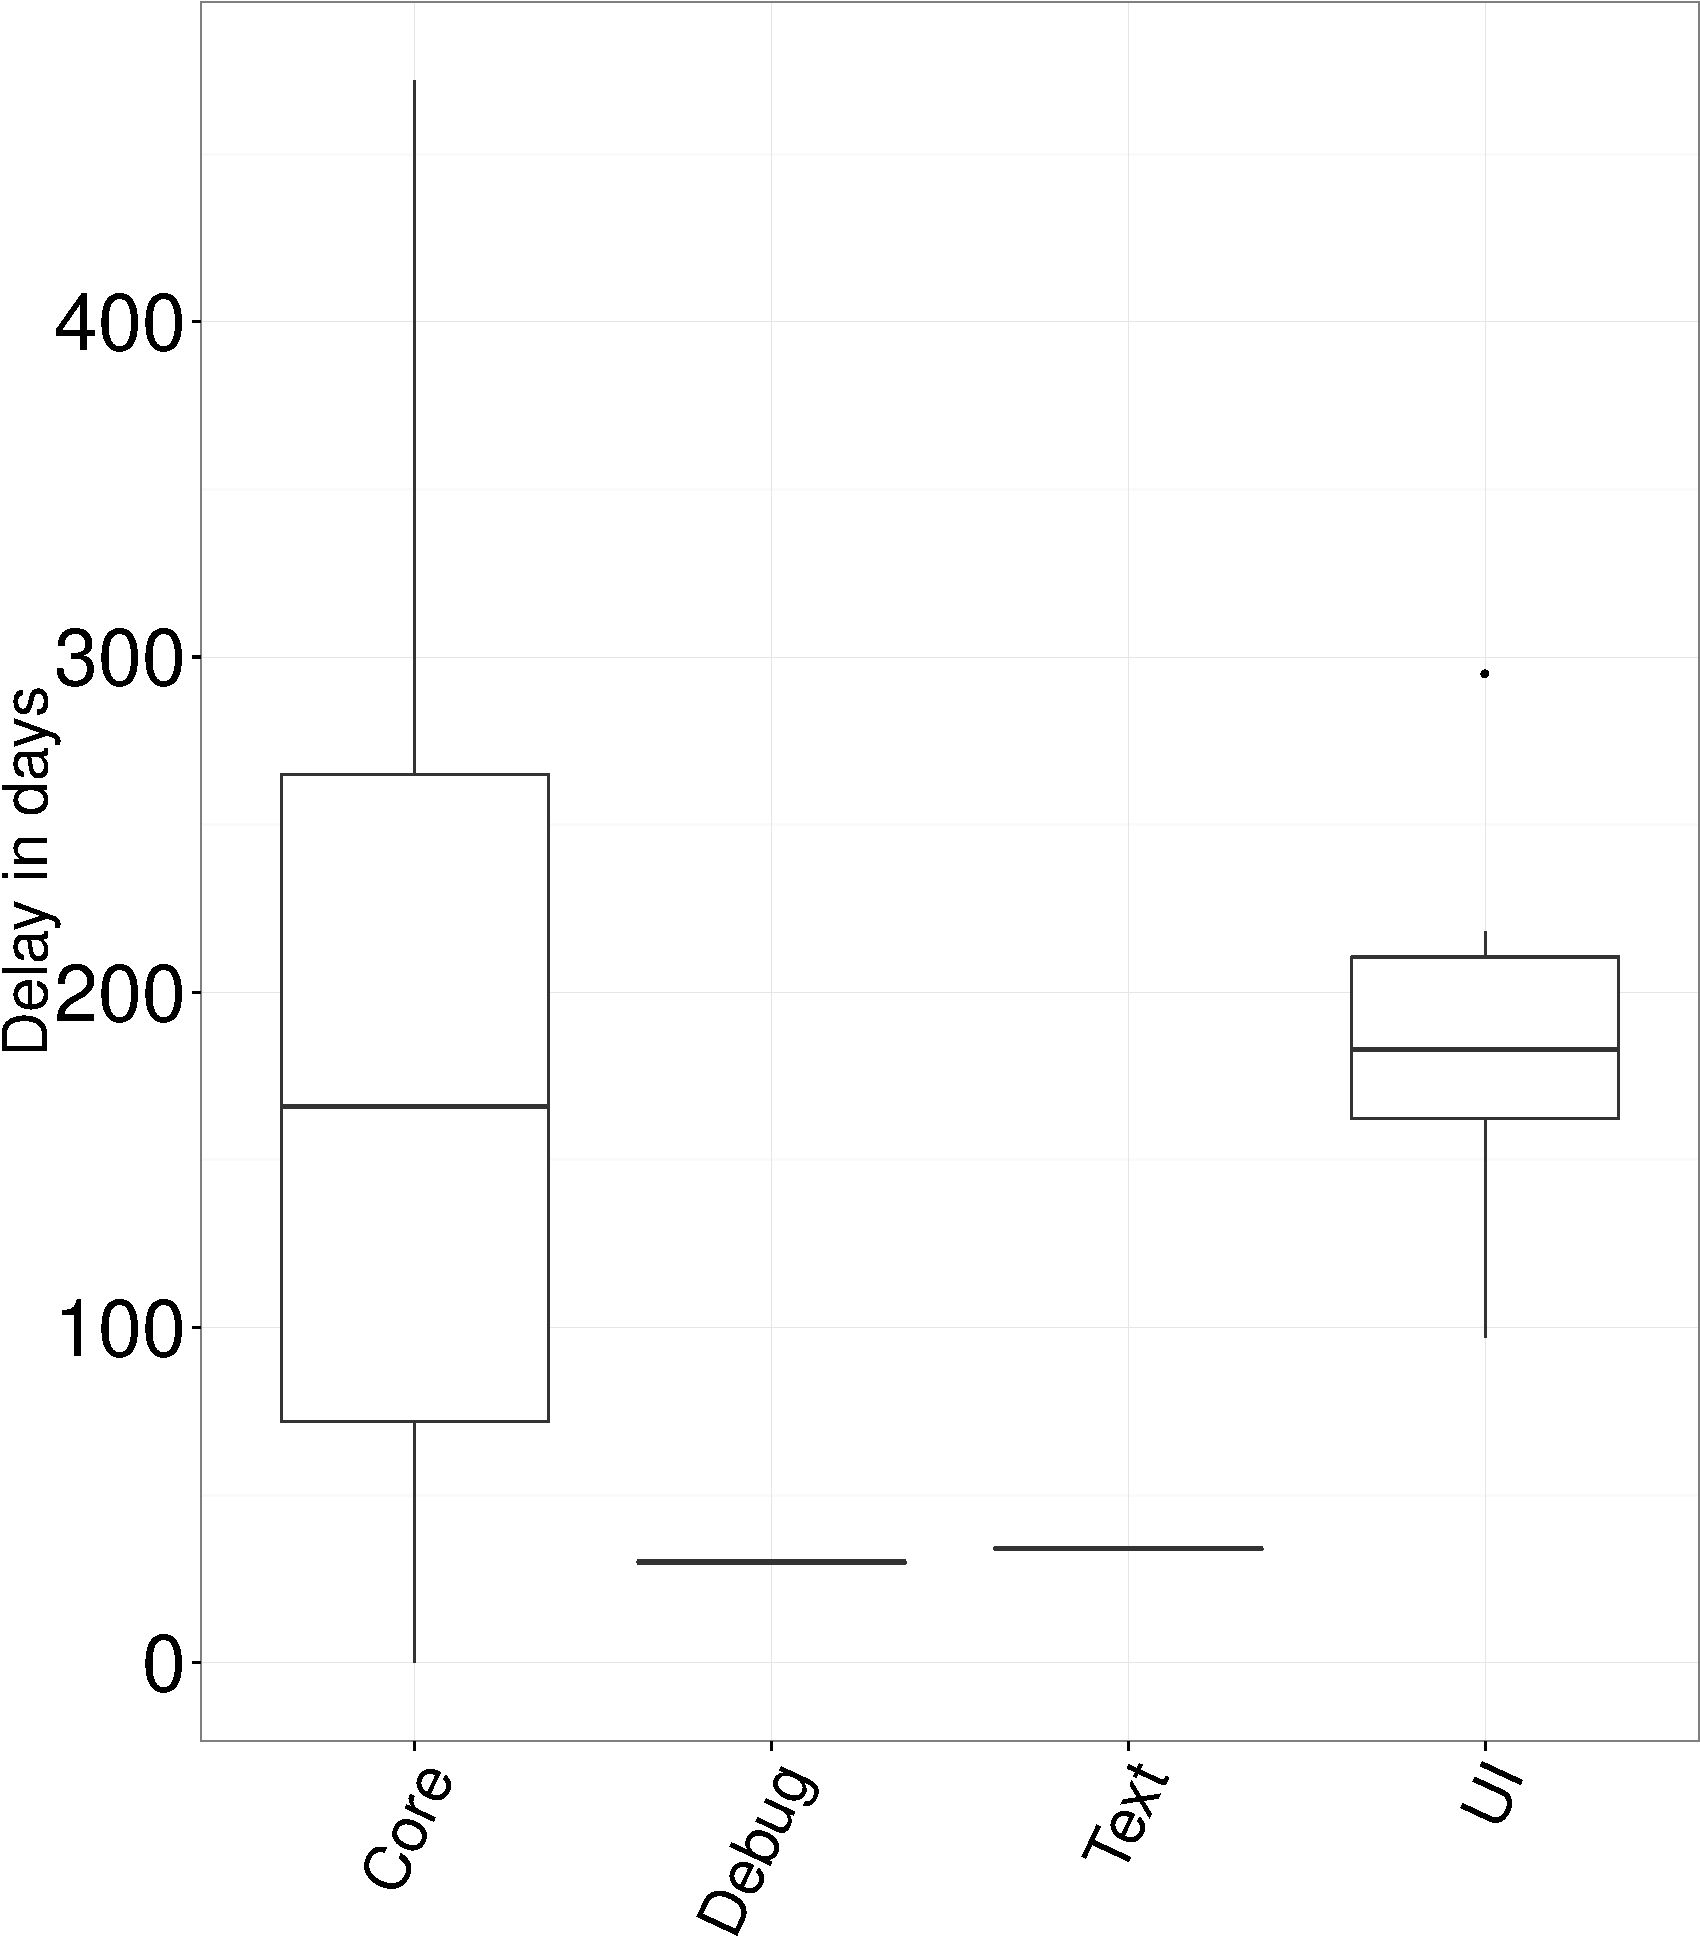
\includegraphics[width=0.40\textwidth,keepaspectratio]
		{chapters/chapter4/figures/components_eclipse.pdf}
	}

	\subfloat[Firefox]{
		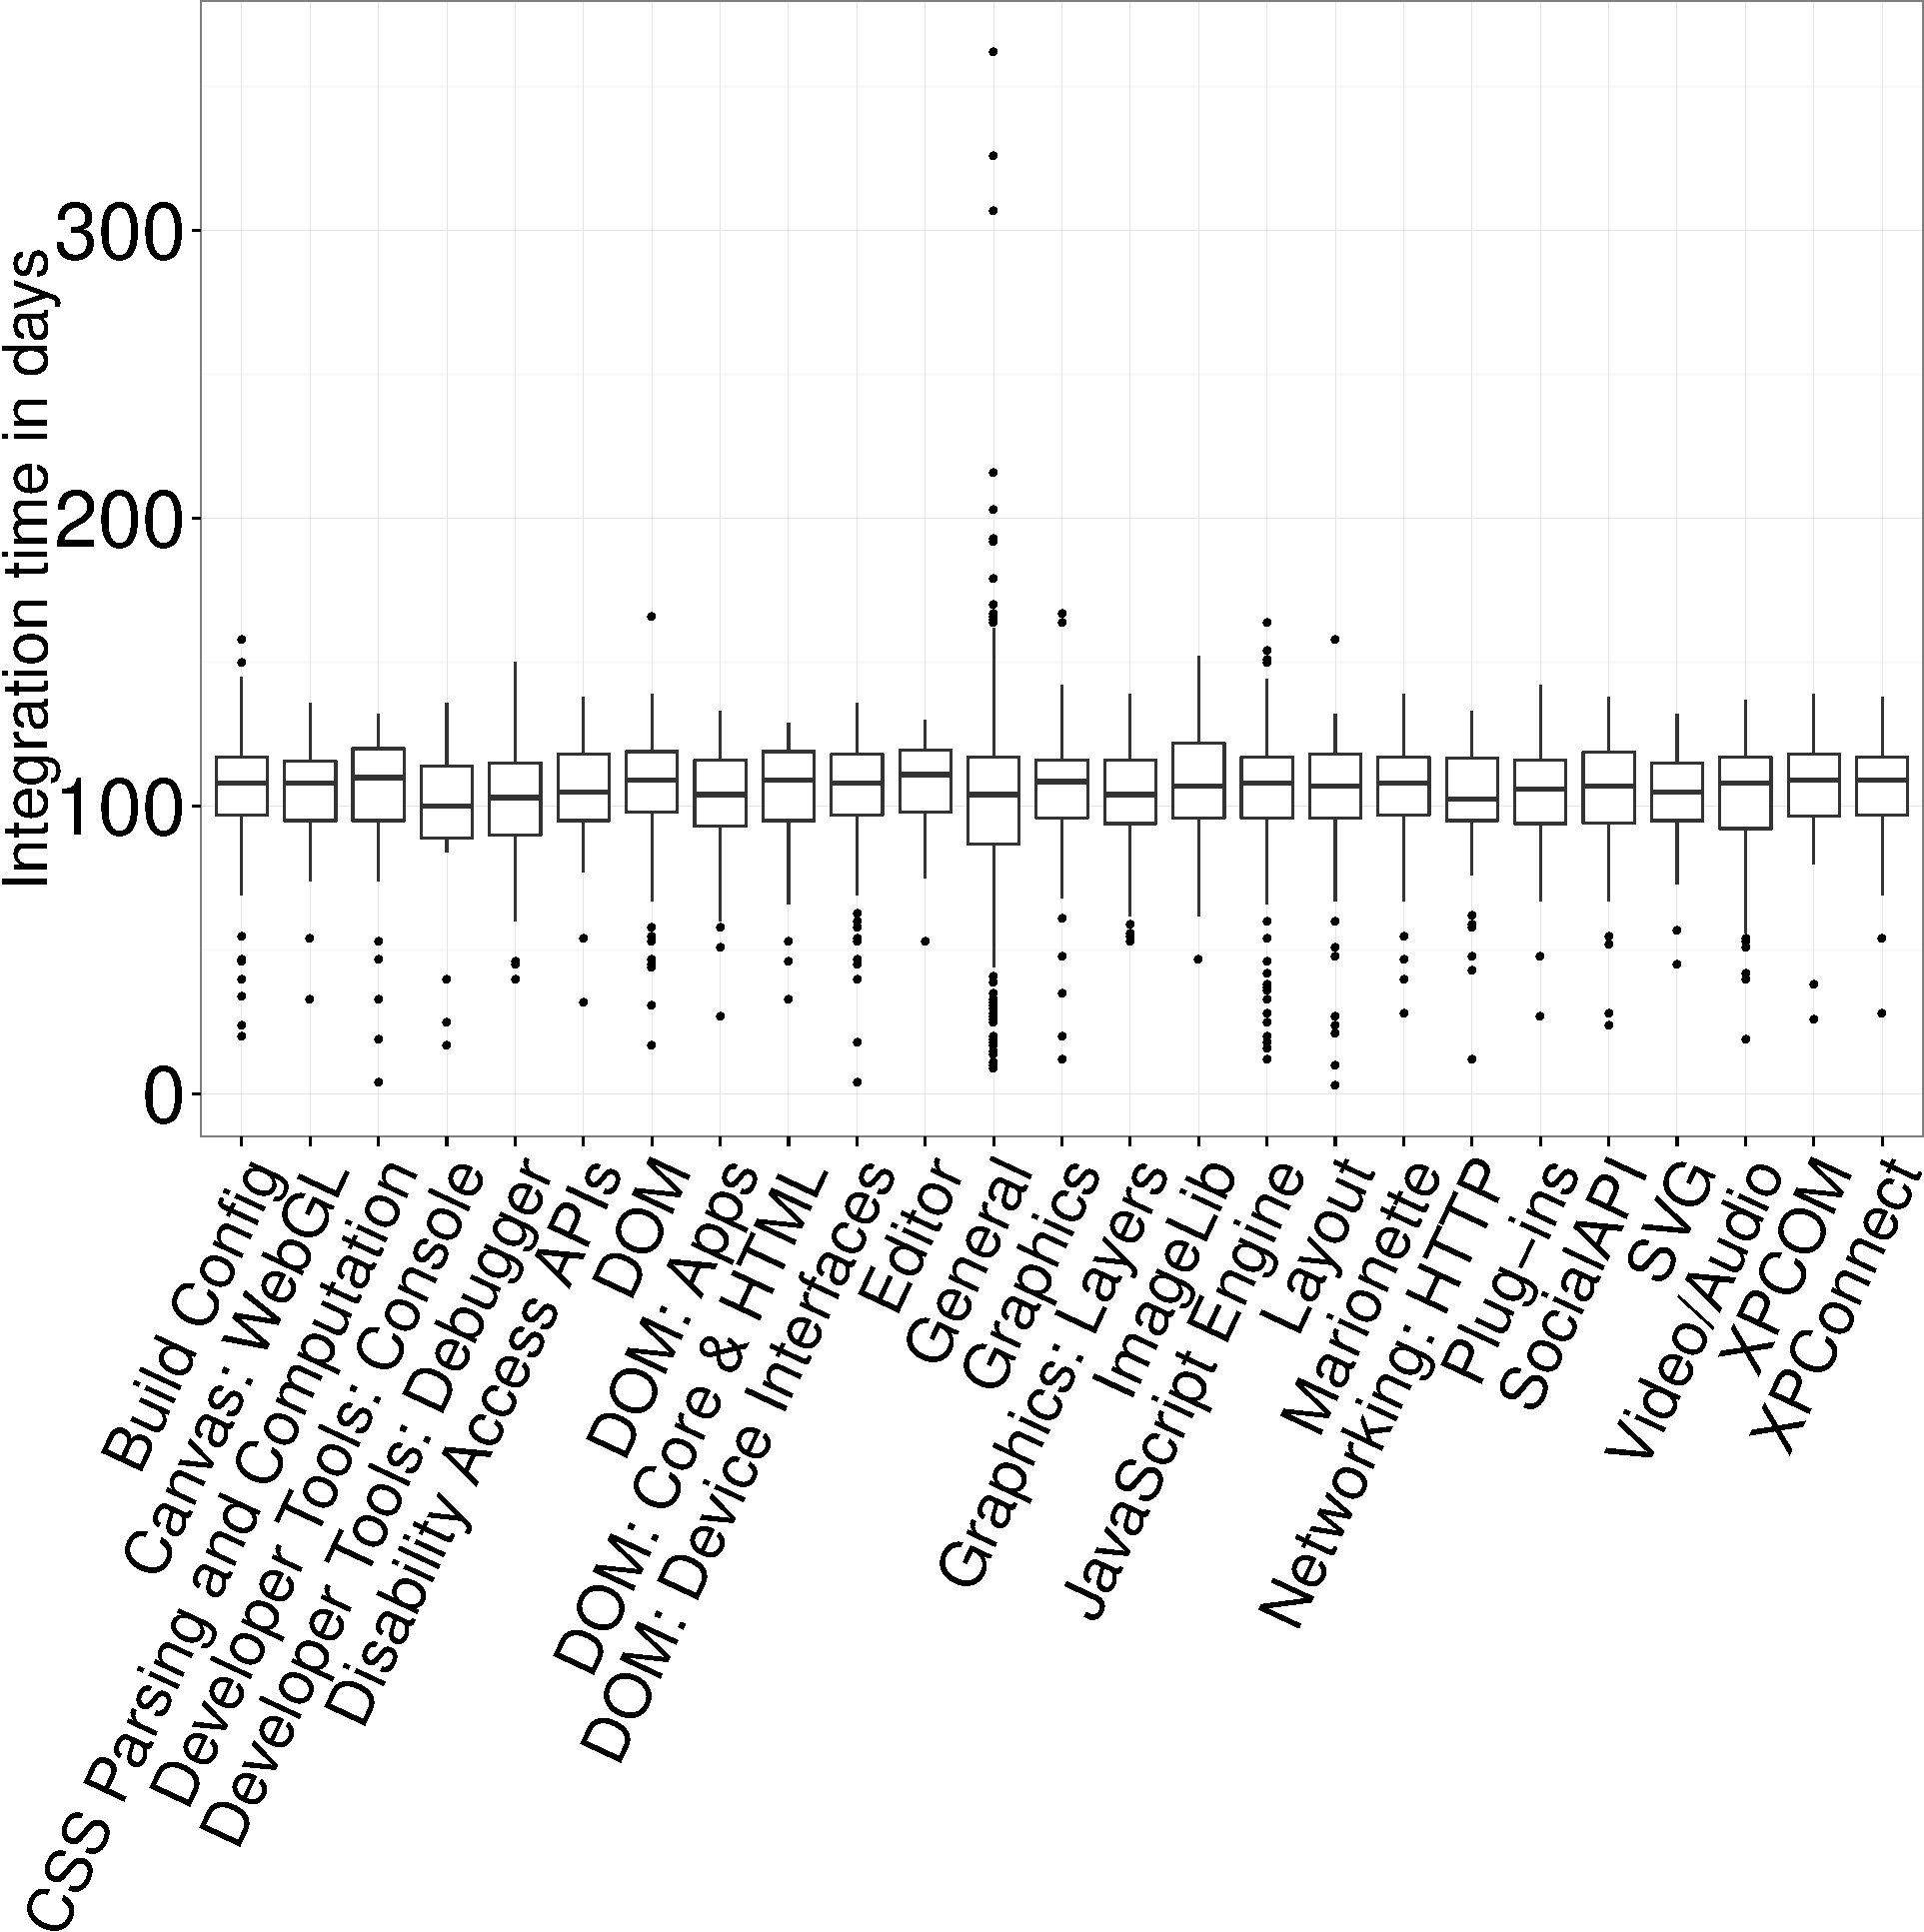
\includegraphics[width=0.40\textwidth,keepaspectratio]
		{chapters/chapter4/figures/components_firefox.pdf}
	}

	\subfloat[ArgoUML]{
		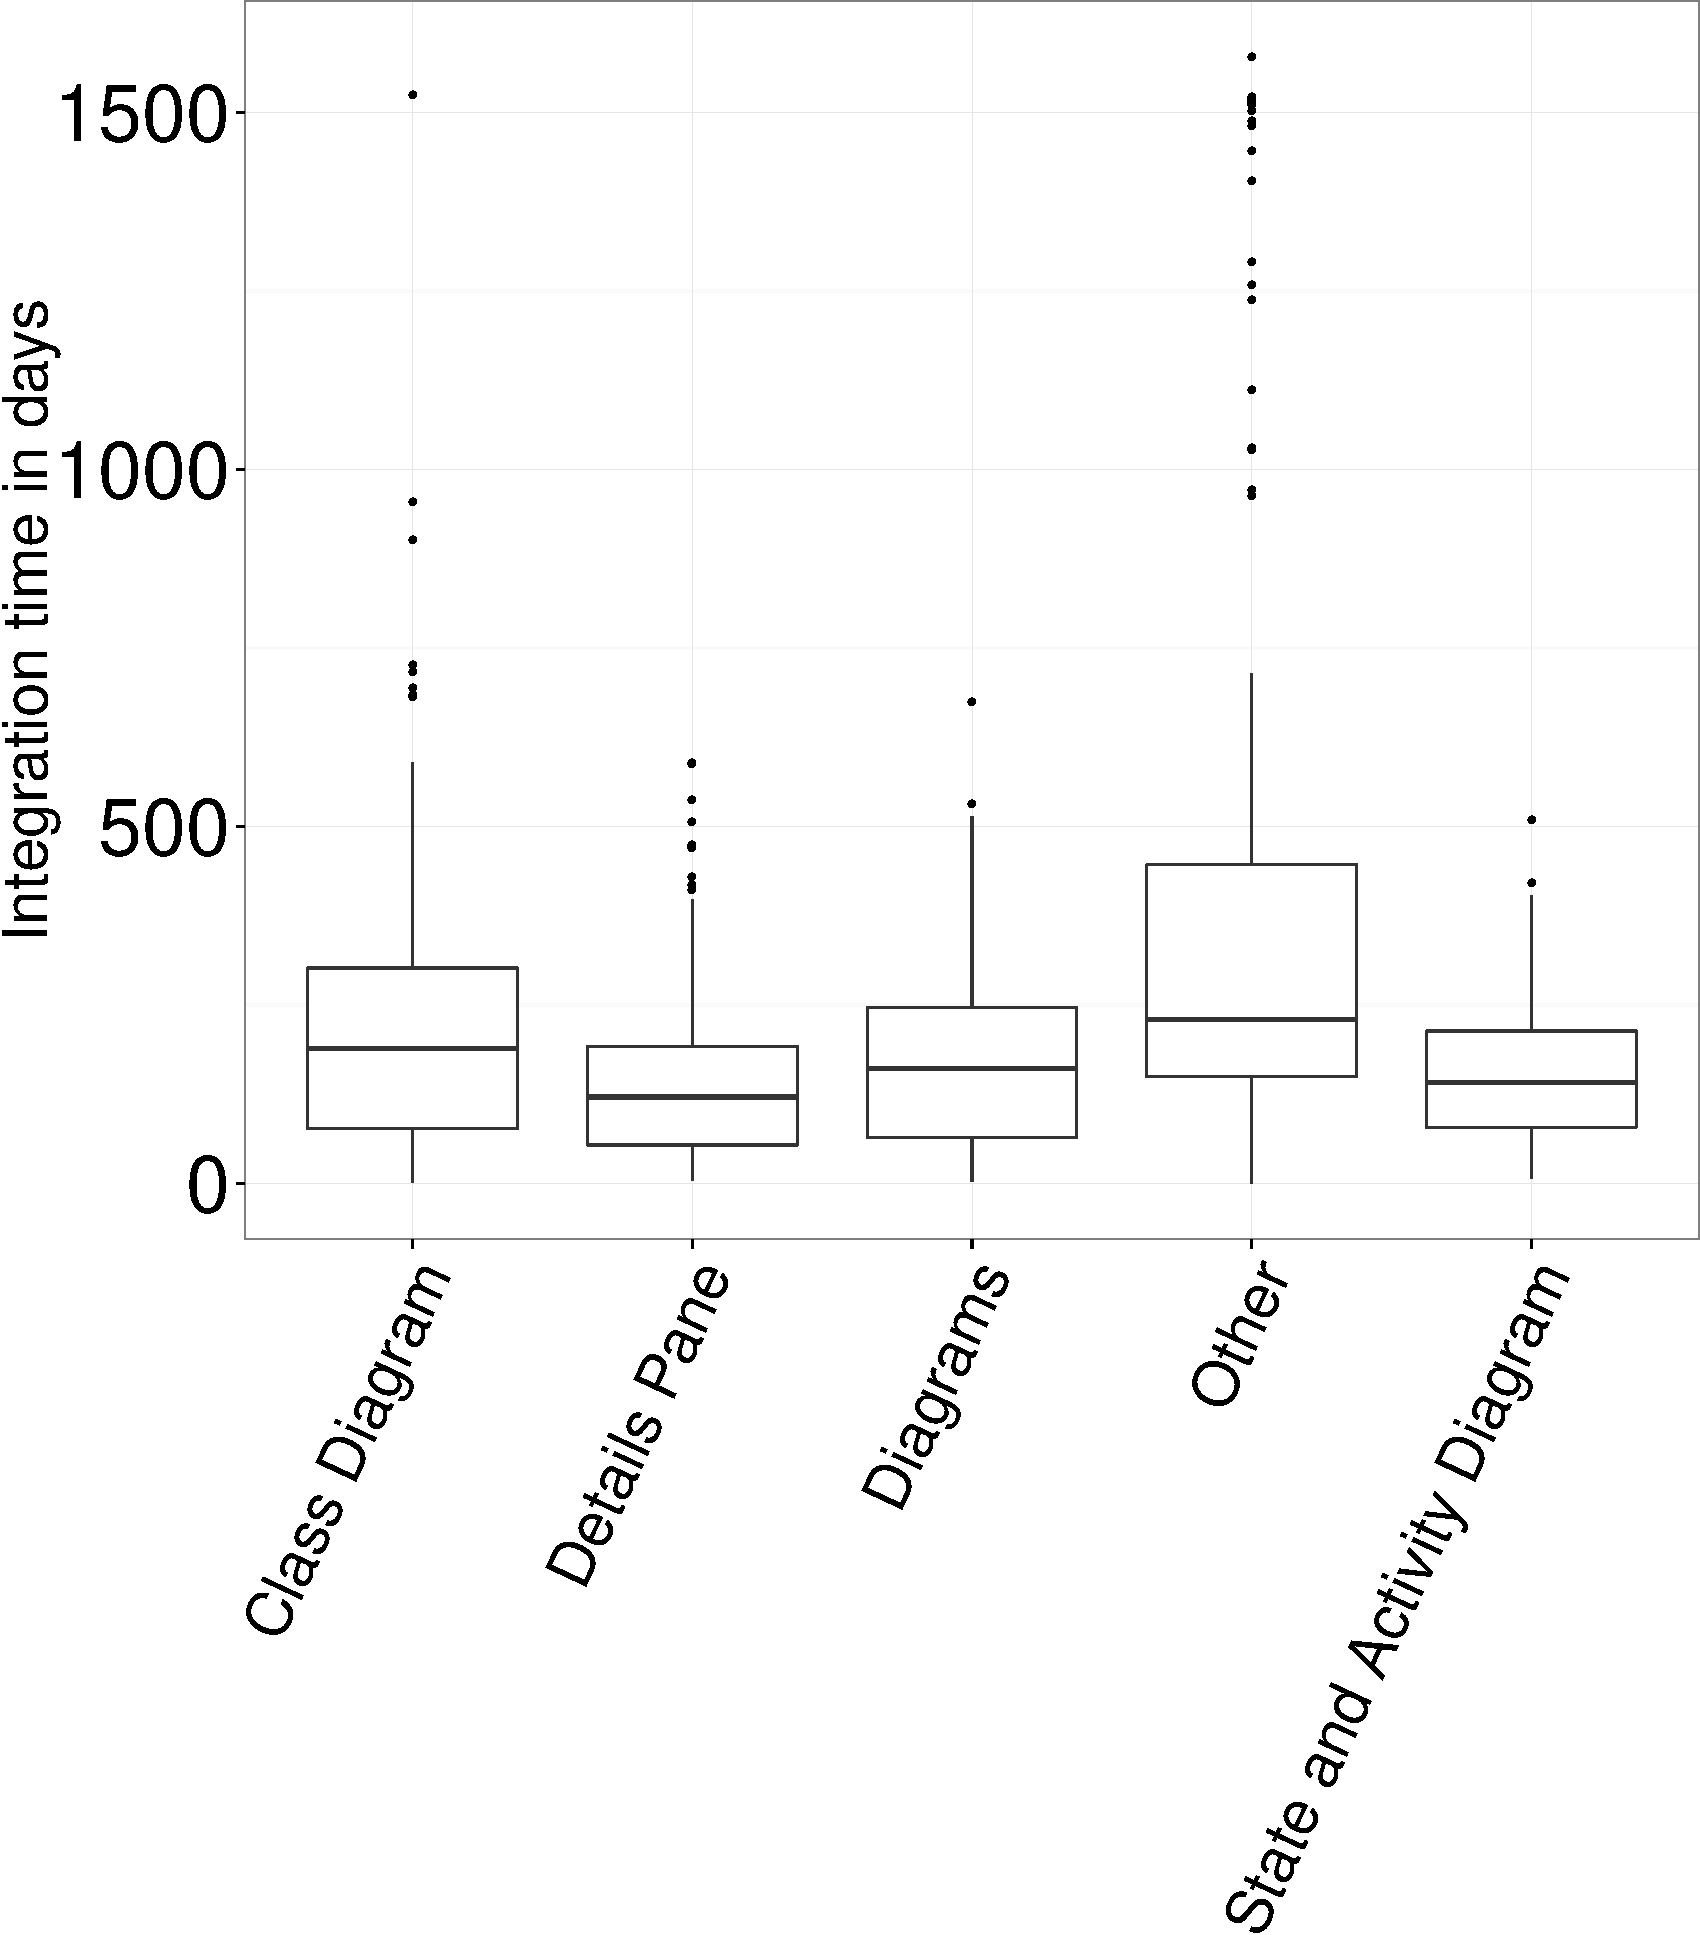
\includegraphics[width=0.40\textwidth,keepaspectratio]
		{chapters/chapter4/figures/components_argouml.pdf}
	}
	\caption{\textbf{Delivery delay per component.} The Figure shows the
		distributions of delivery delay in terms of days for each
		component of the studied projects.
	}
	\label{ch4:fig:component_analysis}
\end{figure}

\noindent\textbf{\textit{The component to which an issue is addressed has little
impact in the delivery delay in terms of days.}} To demonstrate this, we group
each addressed issue according to the components that such an issue modifies. We use
components that have at least 100 addressed issues as a threshold for our analysis.
We then compare the distribution of delivery delay in terms of days in these
components.
\hyperref[ch4:fig:component_analysis]{Figure}~\ref{ch4:fig:component_analysis} shows the
distributions of delivery delay in terms of days per component. We do not
observe a considerable difference between distributions of delivery delay in
the ArgoUML or Firefox projects. The distribution of the ``Other'' component in
the ArgoUML project is more skewed, which is suggestive of its generic
role---such a component may encompass a more broad spectrum of addressed issues. On
the other hand, 99\% of the addressed issues in the Eclipse (JDT) project belong to
the ``Core'' component (thus its skewness). Finally, the ``Debug'' and ``Text''
Eclipse components contain only one addressed issue each.   

\conclusionbox{The workload in terms of backlog of issues awaiting integration
	and the integration speed of prior addressed issues of a given resolver play
	a important role to model delivery delay in terms of days. Moreover,
	the initial \textit{queue position} is the most important attribute in
	all models that we fit to study delivery delay in terms of days.}

